\documentclass[../../../../main.tex]{subfiles}
\begin{document}

\section*{第1問}

% (手書き解答なし)

\section*{第2問}

[解] $a_2 = 2, a_3 = 4, a_4 = 8 \quad \dots \text{①}$

「 $a_n = 2^n \quad \dots \text{②}$ が任意の $n \in \mathbb{N}$ で成りたつこと 」$\quad \dots \text{③}$
を帰納的に示す。$n=1$ の時は成立。$n \leqq k$ での成立を仮定する
($k \in \mathbb{N}$) と、$2$進数表示をかんがえて、$T = \underbrace{111\dots1}_{k+1}$ から $1$ まで
の数を全てつくることができるから、
\[
a_{k+1} = T + 1 = 2^{k+1}
\]
よって $n = k+1$ でも ② は成立

以上より ③ が示されたので、$a_n = 2^n$ である。

[別] 「 $1, 2, \dots, 2^n$ を用いて、$1 \sim 2^{n+1}-1$ を全てつくれること 」を
帰納的に示す。$n=k$ で仮定する。$1, 2, \dots, 2^{k+1}$ について
$1 \sim 2^{k+1}-1$ は仮定よりつくれるから、
\[
\begin{cases}
1^\circ & 2^{k+1} \text{ はつくれる} \\
2^\circ & 2^{k+1}+1, \dots, 2^{k+2}-1 \text{ は } 2^{k+1} \text{ を加えてつくれる}
\end{cases}
\]
よって $n = k+1$ でも成立。

\section*{第3問}

\begin{center}
\begin{tikzpicture}[scale=1.8, >=stealth]
    % Axes
    \draw[->] (0,0) -- (2.5,0) node[right] {$y$};
    \draw[->] (0,0) -- (0,2.5) node[left] {$z$};
    \draw[->] (0,0) -- (-1.2,-1.2) node[below left] {$x$};
    \node[below left] at (0,0) {$O$};

    % Circle C
    \draw[dashed] (0,0) ellipse (1.0 and 0.4);
    \node[left] at (-0.8, 0.2) {$C$};

    % Point A
    \coordinate (A) at (1.3,0);
    \fill (A) circle (1.2pt) node[below] {$A$};

    % Line l through A
    \draw[thick] (0.3, 2.2) -- (2.3, -1.2) node[right] {$l$};

    % Angle pi/4
    \draw (1.3,0) ++(115:0.5) arc (115:150:0.5);
    \node at (0.9, 1.6) {$\pi/4$};
\end{tikzpicture}
\end{center}

[解] $A(0, a, 0)$ とする。この時、$l$ の方向ベクトル $\vec{v}$ は
$\vec{v} = \begin{pmatrix} 1 \\ 0 \\ -1 \end{pmatrix}$ と書けるから、$l$ 上の点 $X$ として
\[
\vec{OX} = \begin{pmatrix} 0 \\ a \\ 0 \end{pmatrix} + t \begin{pmatrix} 1 \\ 0 \\ -1 \end{pmatrix} \quad (t \in \mathbb{R})
\]
とできる。又、$C = \cos\theta, S = \sin\theta \ (0 \leqq \theta < 2\pi)$ とすると、
$C$ 上の点 $P$ は $P(C, S, 0)$ とかける。以下対称性から $t > 0$ として考える。

\begin{align*}
\overline{PX}^2 &= (t - C)^2 + (a - S)^2 + t^2 \\
&= (2t^2 + a^2 + 1) - 2(t C + a S) \quad \dots \text{①}
\end{align*}

$t, a > 0$ だから、コーシー・シュワルツから
\[
t C + a S \leqq \sqrt{t^2 + a^2}
\]
等号成立は $\begin{pmatrix} C \\ S \end{pmatrix} \mathbin{/\!\!/} \begin{pmatrix} t \\ a \end{pmatrix}$ の時である。したがって、①の最小値は
\[
\overline{PX}^2 = (2t^2 + a^2 + 1) - 2\sqrt{t^2 + a^2} \equiv f(p) \quad (p = t^2 \geqq 0)
\]
で与えられる。
\[
f'(p) = 2 - 2 \cdot \frac{1}{2\sqrt{p + a^2}} = \frac{2\sqrt{p + a^2} - 1}{\sqrt{p + a^2}}
\]
から、$a$ によって下表をとる。

\begin{enumerate}
  \item[$1^\circ$] $a \geqq \frac{1}{2}$ の時
  
  $f'(p) \geqq 0$ だから、$f$ は単調増加で、$p = 0$ で $\min \overline{PX}^2 = a^2 - 2a + 1 = (a - 1)^2$
  だから、$\overline{PX} \geqq 0$ より、$\min \overline{PX} = |a - 1|$

  \item[$2^\circ$] $0 < a \leqq \frac{1}{2}$ の時
  
  下表をとる。
  \[
  \begin{array}{c|c|c|c|c}
  p & 0 & \dots & \frac{1}{4} - a^2 & \dots \\ \hline
  f' & & - & 0 & + \\ \hline
  f & & \searrow & & \nearrow
  \end{array}
  \]
  したがって、$p = \frac{1}{4} - a^2$ で $\min \overline{PX}^2 = \frac{1}{2} - a^2 \quad \therefore \min \overline{PX} = \sqrt{\frac{1}{2} - a^2}$ となる。
\end{enumerate}

以上から、
\[
\min \overline{PX} = \begin{cases}
\sqrt{\frac{1}{2} - a^2} & \left(0 < a \leqq \frac{1}{2}\right) \\
|a - 1| & \left(\frac{1}{2} \leqq a\right)
\end{cases}
\quad \text{/\!\!/}
\]

[解2] (①以下)
\begin{align*}
\overline{PX}^2 &= 2\left(t - \frac{C}{2}\right)^2 + a^2 - 2a S + 1 - \frac{S^2}{2} \\
&\geqq \frac{C^2 - 1}{2} - 2a S + a^2 + 1 \quad \left(\text{等号成立は } t = \frac{C}{2}\right) \\
&= \frac{1}{2}(C - 2a)^2 - a^2 + \frac{1}{2}
\end{align*}
だから、$0 \leqq a \leqq \frac{1}{2}$ の時、$\min \overline{PX}^2 = \frac{1}{2} - a^2$ となる。(以下略)
\[
\frac{1}{2} \leqq a \text{ の時、} \min \overline{PX}^2 = (a - 1)^2 \quad \text{/\!\!/}
\]

\section*{第4問}

\begin{center}
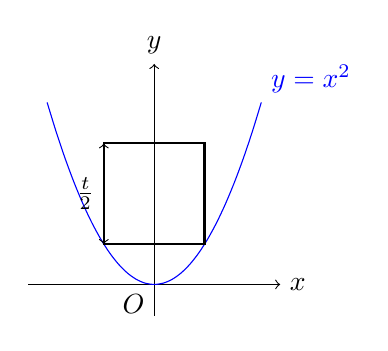
\begin{tikzpicture}[scale=0.8]
    % Parabola y = x^2
    \draw[->] (-2,0) -- (2,0) node[right] {$x$};
    \draw[->] (0,-0.5) -- (0,3.5) node[above] {$y$};
    \draw[domain=-1.7:1.7, smooth, variable=\x, blue] plot ({\x}, {\x*\x}) node[above right] {$y=x^2$};
    
    % Square 1
    \draw[thick] (-0.8, 0.64) -- (0.8, 0.64) -- (0.8, 2.24) -- (-0.8, 2.24) -- cycle;
    \draw[<->] (-0.8, 0.64) -- (-0.8, 2.24) node[midway, left] {$\frac{t}{2}$};
    \node[below left] at (0,0) {$O$};
\end{tikzpicture}
\qquad
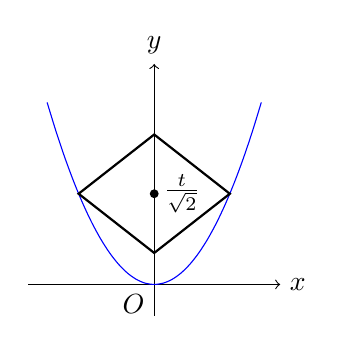
\begin{tikzpicture}[scale=0.8]
    % Parabola y = x^2
    \draw[->] (-2,0) -- (2,0) node[right] {$x$};
    \draw[->] (0,-0.5) -- (0,3.5) node[above] {$y$};
    \draw[domain=-1.7:1.7, smooth, variable=\x, blue] plot ({\x}, {\x*\x});
    
    % Diamond Square 2
    \draw[thick] (0, 0.5) -- (1.2, 1.44) -- (0, 2.38) -- (-1.2, 1.44) -- cycle;
    \fill (0,1.44) circle (2pt) node[right] {$\frac{t}{\sqrt{2}}$};
    \node[below left] at (0,0) {$O$};
\end{tikzpicture}
\qquad
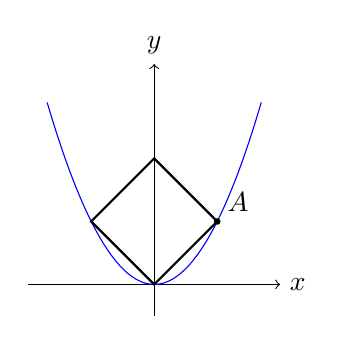
\begin{tikzpicture}[scale=0.8]
    % Parabola y = x^2
    \draw[->] (-2,0) -- (2,0) node[right] {$x$};
    \draw[->] (0,-0.5) -- (0,3.5) node[above] {$y$};
    \draw[domain=-1.7:1.7, smooth, variable=\x, blue] plot ({\x}, {\x*\x});
    
    % Diamond Square 3 at Origin
    \draw[thick] (0,0) -- (1, 1) node[above right] {$A$} -- (0, 2) -- (-1, 1) -- cycle;
    \fill (1,1) circle (1.5pt);
\end{tikzpicture}
\end{center}

[解] 中心が $y$ 軸上にないものは、中心が $y$ 軸上にくるよう平行移動することで、より $y$ 座標を小さくできるから、中心が $y$ 軸上にあるもののみ考える。この時、$y$ 座標が最小になるのは、以下のいずれか

\begin{enumerate}
  \item[$1^\circ$] 正方形の下2辺が $y=x^2$ にある
  \item[$2^\circ$] 正方形の対角線上の点2つが $y=x^2$ にある
  \item[$3^\circ$] 1つの頂点が原点にある
\end{enumerate}

以下、$y$ 座標 $f(t)$ とおく。($t > 0$)

$1^\circ$ の時
\[
f_1(t) = \left(\frac{t}{2}\right)^2 + \frac{t}{2} = \frac{1}{4}t^2 + \frac{1}{2}t
\]

$2^\circ$ の時
\[
f_2(t) = \left(\frac{t}{\sqrt{2}}\right)^2
\]
であり、この時、一番下の頂点 $(0, f(t) - \frac{t}{\sqrt{2}})$ が原点より上にあることが必要で、
\[
f(t) - \frac{t}{\sqrt{2}} = \frac{t}{2}\cdot t - \frac{t}{\sqrt{2}} = \frac{t}{\sqrt{2}}\left(\frac{t}{\sqrt{2}} - 1\right) \geqq 0 \iff t \geqq \sqrt{2} \quad (\because t > 0)
\]

$3^\circ$ の時、
\[
f_3(t) = \frac{t}{\sqrt{2}}
\]
であり、この時、$3^\circ$ の図の $A$ が $y=x^2$ に含まれていることが必要で、
\[
\frac{t}{\sqrt{2}} \geqq \left(\frac{t}{\sqrt{2}}\right)^2 \iff 0 < t \leqq \sqrt{2}
\]

以上のうち、$\min$ のものがもとめる関数である。これらを図示して右上図を得る

\begin{center}
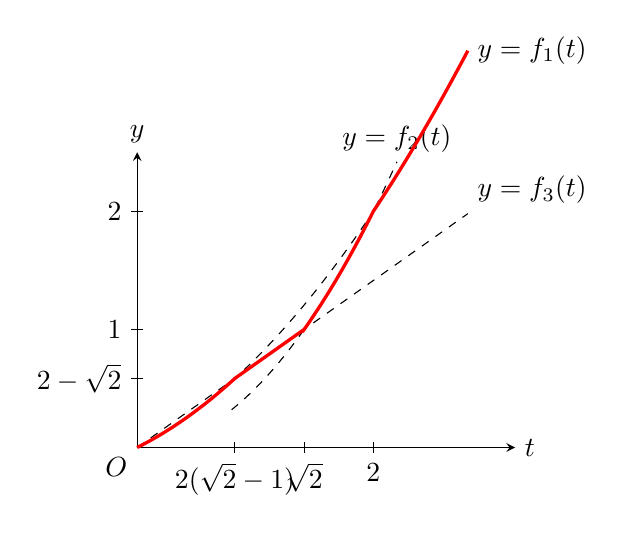
\begin{tikzpicture}[scale=1.5, >=stealth]
    \draw[->] (0,0) -- (3.2,0) node[right] {$t$};
    \draw[->] (0,0) -- (0,2.5) node[above] {$y$};
    \node[below left] at (0,0) {$O$};

    % Points on t-axis
    \draw (0.828, 0.05) -- (0.828, -0.05) node[below] {$2(\sqrt{2}-1)$};
    \draw (1.414, 0.05) -- (1.414, -0.05) node[below] {$\sqrt{2}$};
    \draw (2.0, 0.05) -- (2.0, -0.05) node[below] {$2$};

    % Values on y-axis
    \draw (0.05, 0.586) -- (-0.05, 0.586) node[left] {$2-\sqrt{2}$};
    \draw (0.05, 1.0) -- (-0.05, 1.0) node[left] {$1$};
    \draw (0.05, 2.0) -- (-0.05, 2.0) node[left] {$2$};

    % Curves
    \draw[dashed, domain=0:2.8, smooth, variable=\t] plot ({\t}, {0.25*\t*\t + 0.5*\t}) node[right] {$y=f_1(t)$};
    \draw[dashed, domain=0:2.8, smooth, variable=\t] plot ({\t}, {\t/1.414}) node[above right] {$y=f_3(t)$};
    \draw[dashed, domain=0.8:2.2, smooth, variable=\t] plot ({\t}, {0.5*\t*\t}) node[above] {$y=f_2(t)$};

    % Thick lower envelope f(t)
    \draw[very thick, red] (0,0) 
        -- plot[domain=0:0.828, smooth, variable=\t] ({\t}, {0.25*\t*\t + 0.5*\t})
        -- plot[domain=0.828:1.414, smooth, variable=\t] ({\t}, {\t/1.414})
        -- plot[domain=1.414:2.0, smooth, variable=\t] ({\t}, {0.5*\t*\t})
        -- plot[domain=2.0:2.8, smooth, variable=\t] ({\t}, {0.25*\t*\t + 0.5*\t});
\end{tikzpicture}
\end{center}

よって求める関数は
\[
f(t) = \begin{cases}
\frac{t}{\sqrt{2}} & (2(\sqrt{2}-1) \leqq t \leqq \sqrt{2}) \\
\frac{1}{2} t^2 & (\sqrt{2} \leqq t \leqq 2) \\
\frac{1}{4} t^2 + \frac{1}{2} t & (0 < t \leqq 2(\sqrt{2}-1), \ 2 \leqq t)
\end{cases}
\quad \text{/\!\!/}
\]
である

\section*{第5問}

\begin{center}
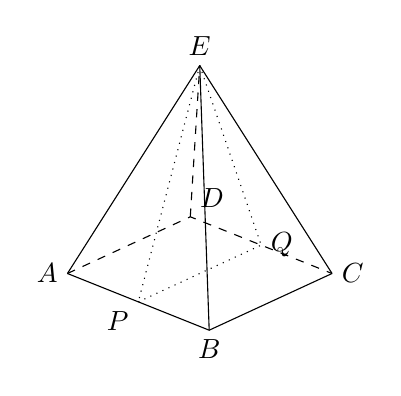
\begin{tikzpicture}[scale=1.2, >=stealth]
    % Square Pyramid E-ABCD
    \coordinate (A) at (-1, 0);
    \coordinate (B) at (0.5, -0.6);
    \coordinate (C) at (1.8, 0);
    \coordinate (D) at (0.3, 0.6);
    \coordinate (E) at (0.4, 2.2);

    \draw[dashed] (A) -- (D) -- (C);
    \draw (A) -- (B) -- (C);
    \draw (A) -- (E);
    \draw (B) -- (E);
    \draw (C) -- (E);
    \draw[dashed] (D) -- (E);

    \node[left] at (A) {$A$};
    \node[below] at (B) {$B$};
    \node[right] at (C) {$C$};
    \node[above right] at (D) {$D$};
    \node[above] at (E) {$E$};

    % Midpoints P and Q
    \coordinate (P) at (-0.25, -0.3);
    \coordinate (Q) at (1.05, 0.3);
    \draw[dotted] (E) -- (P);
    \draw[dotted] (E) -- (Q);
    \draw[dotted] (P) -- (Q);
    \node[below left] at (P) {$P$};
    \node[right] at (Q) {$Q$};
\end{tikzpicture}
\qquad
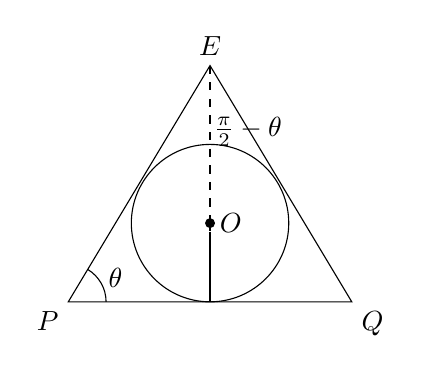
\begin{tikzpicture}[scale=1.2, >=stealth]
    % Triangle EPQ
    \coordinate (P) at (-1.5, 0);
    \coordinate (Q) at (1.5, 0);
    \coordinate (E) at (0, 2.5);

    \draw (P) -- (Q) -- (E) -- cycle;
    \node[below left] at (P) {$P$};
    \node[below right] at (Q) {$Q$};
    \node[above] at (E) {$E$};

    % Inscribed circle radius 1
    \coordinate (O) at (0, 0.833);
    \draw (O) circle (0.833);
    \fill (O) circle (1.5pt) node[right] {$O$};
    \draw[dashed] (O) -- (0,0);
    \draw[dashed] (E) -- (0,0);

    % Angle labels
    \draw (P) ++(0:0.4) arc (0:59:0.4);
    \node at (-1.0, 0.25) {$\theta$};

    \node at (0.4, 1.8) {$\frac{\pi}{2}-\theta$};
\end{tikzpicture}
\end{center}

[解] $S$ の半径に規格化して考える。$V$ の底辺の長さを $x$ とする。

右のように各点を定める。($P, Q$ は辺の中点) $E, P, Q$ を含む平面で切ると、対称性から、この平面内に $S$ の中心 $O$ が含まれ、右下の図のようになる。$\angle EPQ = \theta$ とする $(0 < \theta < \pi/2)$

\[
\overline{PQ} = \frac{2}{\tan \frac{\theta}{2}} \quad \dots \text{①}
\]
\[
EQ = \frac{\frac{1}{2}\overline{PQ}}{\cos \theta} = \frac{1}{\tan \frac{\theta}{2} \cdot \cos \theta} \quad \dots \text{②}
\]
だから、$t = \tan \frac{\theta}{2} \ (0 < t < 1)$ とすると、
\[
\begin{cases}
x = \frac{2}{t} \\
EQ = \frac{1+t^2}{t(1-t^2)}
\end{cases}
\quad \dots \text{③}
\]
である。$V, S$ の表面積を各々 $T_1, T_2$ とすると、
\begin{align*}
T_1 &= \text{□}ABCD + 4 \Delta ECD \\
&= x^2 + 2x \cdot EQ \\
&= \frac{4}{t} \left( \frac{1}{t} + \frac{2(1+t^2)}{t(1-t^2)} \right) \\
&= \left(\frac{2}{t}\right)^2 \frac{2}{1-t^2} \quad \dots \text{④}
\end{align*}
\[
T_2 = 4\pi \quad \dots \text{⑤}
\]
だから、④⑤より
\[
R = \frac{T_2}{T_1} = \frac{4\pi}{\frac{8}{t^2(1-t^2)}} = \frac{\pi}{2} t^2(1-t^2) \leqq \frac{\pi}{2} \cdot \frac{1}{4} = \frac{\pi}{8} \quad \left(\text{等号成立は } t = \frac{1}{\sqrt{2}} \ (0 < t < 1) \text{ を満たす}\right)
\quad \text{/\!\!/}
\]

\section*{第6問}

% (手書き解答なし)

\end{document}
